%---------------------------------------------------------------------------
% System use cases.
%
%---------------------------------------------------------------------------


\section{Use cases}
\label{sec:ch4_usecases}

System use cases have been divided into three functional parts. Each of those parts is related to specific functional
block, related to: resources, measurements and visualizations. For each block, diagram in UML notation with additional
description is provided. This approach is equal to the second level of detail in writing use cases, as proposed by A.
Cockburn\cite{0201702258}. 

Because system isn't expected to work with sensitive information, there is no authorization mechanisms or access
control management considered. This also implies, that in all use case diagrams, there is only one actor, namely
user.

\pagebreak

\subsection{Resources Management}
\label{subsec:resources_mgmnt}

Figure \ref{fig:usecase_resources} shows diagram depicting use cases related to resources management. This includes most
generic actions like adding, removing, viewing state. Additionally application gives user ability to manage life cycle
of specific resources (e.g. threads, processes) - user can pause, stop or resume previously paused item. What also
should be mentioned, diagram covers indirect actions that might be performed by user, like selecting which monitoring
hub should be used to manage given resource, connecting to external monitoring hub, or even starting it.

\begin{figure}[ht]
  \centering
  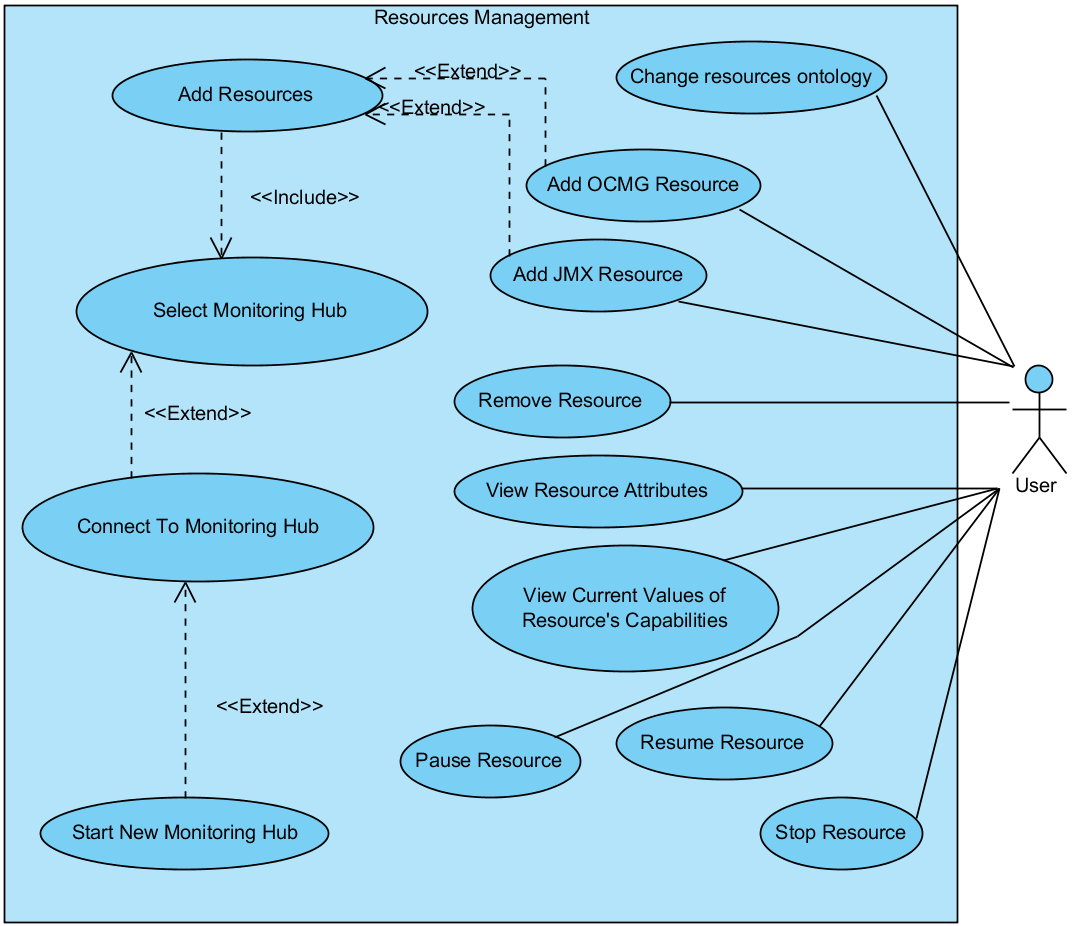
\includegraphics[width=0.8\textwidth]{resources}
  \caption{Resources management use case diagram}
  \label{fig:usecase_resources}
\end{figure}

Main use cases (actions performed by user directly to achieve his/hers aims):

\begin{itemize}
 \item {\bf Add OCMG Resource}~~~~~~~~~~~~~~~~~~~~~~~~~~~~~~~~~~~~~~~~~~~~~~~~~~~~~~~~\linebreak
Adding of OCMG resources. OCMG resource is resources monitored using OCMG monitoring system. This use case is
generalization of Add Resource. User should be able to select which application registered at Main SM to monitor. After
selecting application, all it's resources will be fetched and added to resource tree.
 \item {\bf Add JMX Resource}~~~~~~~~~~~~~~~~~~~~~~~~~~~~~~~~~~~~~~~~~~~~~~~~~~~~~~~~\linebreak
Adding of JMX resources. JMX resource is resource to which Monitoring Hub can connect using SUN's JMX protocol. Adding
JMX resource user selects artificial application with cluster, and specifies URLs that can be used to connect to JVMs
to monitor.
 \item {\bf Remove Resource}~~~~~~~~~~~~~~~~~~~~~~~~~~~~~~~~~~~~~~~~~~~~~~~~~~~~~~~~\linebreak
Every added resource can be simply removed. All it's measurements, and sub resources are removed as well.
 \item {\bf View Resource Attributes} ~~~~~~~~~~~~~~~~~~~~~~~~~~~~~~~~~~~~~~~~~~~~~~~~~~~~~~~~\linebreak
By selecting previously added resource, user should be able to view given resource's static attributes. This is highly
resource-specific. For example, process resource may have attributes like executable path, command line attributes, etc.
 \item {\bf View Current Values of Resource's
Capabilities}~~~~~~~~~~~~~~~~~~~~~~~~~~~~~~~~~~~~~~~~~~~~~~~~~~~~~~~~\linebreak
After selecting previously added resource, user can trigger fetch of all resource's capabilities values and thus view
snapshot of resource's state at 'now' moment of time.
 \item {\bf Pause Resource}~~~~~~~~~~~~~~~~~~~~~~~~~~~~~~~~~~~~~~~~~~~~~~~~~~~~~~~~\linebreak
User should be able to manage resource's life cycle if applicable. Thus, specific resources like threads, processes, or
nodes can be paused, which halts all execution on given resource.
 \item {\bf Resume Resource}~~~~~~~~~~~~~~~~~~~~~~~~~~~~~~~~~~~~~~~~~~~~~~~~~~~~~~~~\linebreak
As stated above, user can pause resource. User also should be able to resume previously paused resource.
 \item {\bf Stop Resource}~~~~~~~~~~~~~~~~~~~~~~~~~~~~~~~~~~~~~~~~~~~~~~~~~~~~~~~~\linebreak
If resource allows it, user should be able to stop given resource totally. After stopping resource, no further
calculations can be performed using given resource, and starting resource again is impossible.
\end{itemize}

Indirect use cases (actions performed by user indirectly to help perform direct actions):

\begin{itemize}
 \item {\bf Add Resource}~~~~~~~~~~~~~~~~~~~~~~~~~~~~~~~~~~~~~~~~~~~~~~~~~~~~~~~~\linebreak
Generalization of Add Jmx Resource and Add OCMG Resource use cases. It was extracted to ease modeling of common
requirements of those use cases - selecting monitoring hub.
 \item {\bf Select Monitoring Hub}~~~~~~~~~~~~~~~~~~~~~~~~~~~~~~~~~~~~~~~~~~~~~~~~~~~~~~~~\linebreak
To be able to add resource, user has to select monitoring hub that will be responsible for managing resources
and gathering data related to them.
 \item {\bf Connect To Monitoring Hub}~~~~~~~~~~~~~~~~~~~~~~~~~~~~~~~~~~~~~~~~~~~~~~~~~~~~~~~~\linebreak
User should be able, to connect to manually started, potentially remote, monitoring hub, prior to selecting one.
 \item {\bf Start New Monitoring Hub}~~~~~~~~~~~~~~~~~~~~~~~~~~~~~~~~~~~~~~~~~~~~~~~~~~~~~~~~\linebreak
User should be able to start new, potentially remote monitoring hub, prior to connecting and using it.
\end{itemize}

\subsection{Measurements Management}
\label{subsec:measurement_mgmnt}


\begin{figure}[ht]
   \centering
   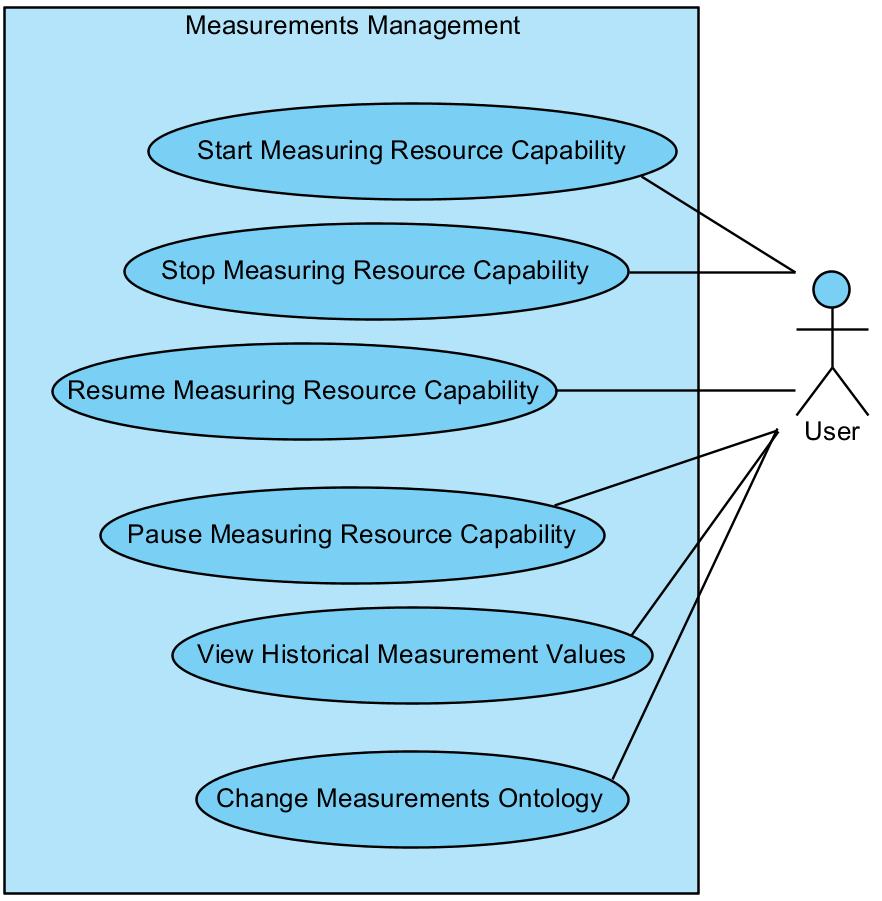
\includegraphics[width=0.5\textwidth]{Measurements}
   \caption{Measurements management use case diagram}
   \label{fig:usecases_measurements}
 \end{figure}

Figure~\ref{fig:usecases_measurements} shows use cases related to measurements management. Measurements functionalities
are a bit simpler then resources management. User is able to start, stop, pause, resume measuring values of given
capabilities. Additionally user can view all historical values, of given measurement.

\subsection{Visualizations Management}
\label{subsec:visualizations_mgmnt}

Figure~\ref{fig:usecases_visualisations} contains diagram of use case allowing management of measurements
visualizations. Regarding visualizations, user can perform following actions:


\begin{itemize}
 \item {\bf Add Visualization}~~~~~~~~~~~~~~~~~~~~~~~~~~~~~~~~~~~~~~~~~~~~~~~~~~~~~~~~\linebreak
User can add new, empty (without any measurements attached) visualization. It is basic step that needs to be done to
visualize measurements.
 \item {\bf Add Measurement To Visualization}~~~~~~~~~~~~~~~~~~~~~~~~~~~~~~~~~~~~~~~~~~~~~~~~~~~~~~~~\linebreak
After creating new visualization, user can add measurements, which makes visualization facility fully functional.
 \item {\bf View Visualization}~~~~~~~~~~~~~~~~~~~~~~~~~~~~~~~~~~~~~~~~~~~~~~~~~~~~~~~~\linebreak
It's most obvious use case - after creating visualization, attaching measurements user can view results of measurements.
 \item {\bf Remove Measurement From Visualization}~~~~~~~~~~~~~~~~~~~~~~~~~~~~~~~~~~~~~~~~~~~~~~~~~~~~~~~~\linebreak
User should be able to remove previously attached measurements from given visualization. This functionality allows full
management of visualizations.~~~~~~~~~~~~~~~~~~~~~~~~~~~~~~~~~~~~~~~~~~~~~~~~~~~~~~~~\linebreak
 \item {\bf Remove Visualization}~~~~~~~~~~~~~~~~~~~~~~~~~~~~~~~~~~~~~~~~~~~~~~~~~~~~~~~~\linebreak
When given visualization isn't needed by user anymore, it can be simply removed from application.
 \item {\bf Edit Visualization Display Options}~~~~~~~~~~~~~~~~~~~~~~~~~~~~~~~~~~~~~~~~~~~~~~~~~~~~~~~~\linebreak
User should be able to have additional level of control over visualizations. Managing plot type allows it - user should
be able to change display type of already created visualization.

\end{itemize}



\begin{figure}[ht]
   \centering
   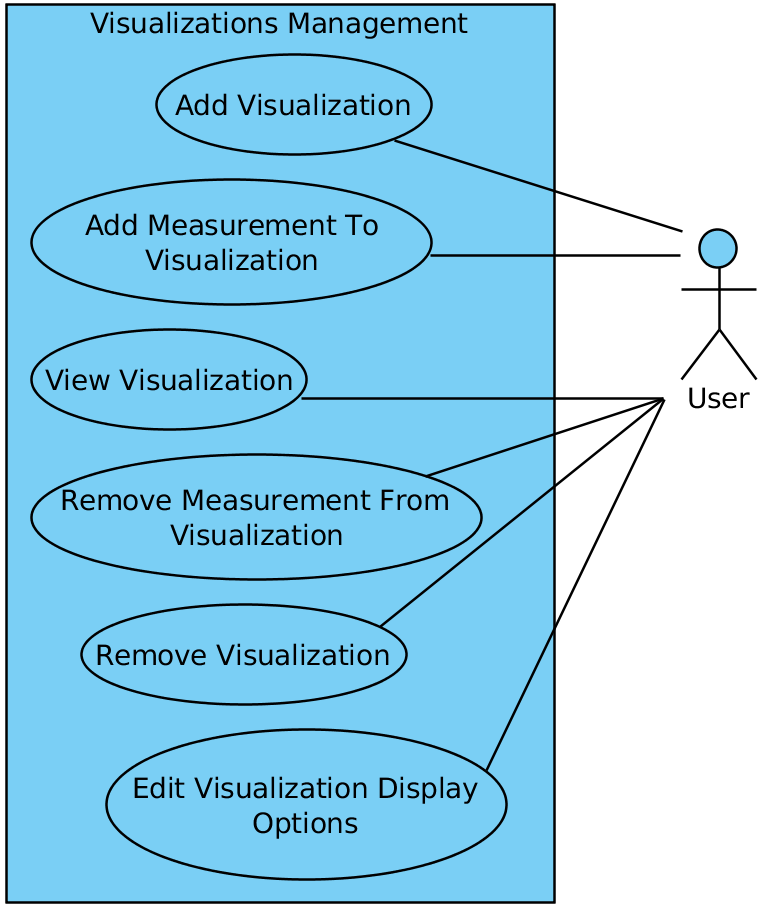
\includegraphics[width=0.4\textwidth]{Visualizations}
   \caption{Visualizations management use case diagram}
   \label{fig:usecases_visualisations}
\end{figure}